% Options for packages loaded elsewhere
\PassOptionsToPackage{unicode}{hyperref}
\PassOptionsToPackage{hyphens}{url}
%
\documentclass[
]{article}
\usepackage{amsmath,amssymb}
\usepackage{lmodern}
\usepackage{iftex}
\ifPDFTeX
  \usepackage[T1]{fontenc}
  \usepackage[utf8]{inputenc}
  \usepackage{textcomp} % provide euro and other symbols
\else % if luatex or xetex
  \usepackage{unicode-math}
  \defaultfontfeatures{Scale=MatchLowercase}
  \defaultfontfeatures[\rmfamily]{Ligatures=TeX,Scale=1}
\fi
% Use upquote if available, for straight quotes in verbatim environments
\IfFileExists{upquote.sty}{\usepackage{upquote}}{}
\IfFileExists{microtype.sty}{% use microtype if available
  \usepackage[]{microtype}
  \UseMicrotypeSet[protrusion]{basicmath} % disable protrusion for tt fonts
}{}
\makeatletter
\@ifundefined{KOMAClassName}{% if non-KOMA class
  \IfFileExists{parskip.sty}{%
    \usepackage{parskip}
  }{% else
    \setlength{\parindent}{0pt}
    \setlength{\parskip}{6pt plus 2pt minus 1pt}}
}{% if KOMA class
  \KOMAoptions{parskip=half}}
\makeatother
\usepackage{xcolor}
\usepackage[margin=1in]{geometry}
\usepackage{color}
\usepackage{fancyvrb}
\newcommand{\VerbBar}{|}
\newcommand{\VERB}{\Verb[commandchars=\\\{\}]}
\DefineVerbatimEnvironment{Highlighting}{Verbatim}{commandchars=\\\{\}}
% Add ',fontsize=\small' for more characters per line
\usepackage{framed}
\definecolor{shadecolor}{RGB}{248,248,248}
\newenvironment{Shaded}{\begin{snugshade}}{\end{snugshade}}
\newcommand{\AlertTok}[1]{\textcolor[rgb]{0.94,0.16,0.16}{#1}}
\newcommand{\AnnotationTok}[1]{\textcolor[rgb]{0.56,0.35,0.01}{\textbf{\textit{#1}}}}
\newcommand{\AttributeTok}[1]{\textcolor[rgb]{0.77,0.63,0.00}{#1}}
\newcommand{\BaseNTok}[1]{\textcolor[rgb]{0.00,0.00,0.81}{#1}}
\newcommand{\BuiltInTok}[1]{#1}
\newcommand{\CharTok}[1]{\textcolor[rgb]{0.31,0.60,0.02}{#1}}
\newcommand{\CommentTok}[1]{\textcolor[rgb]{0.56,0.35,0.01}{\textit{#1}}}
\newcommand{\CommentVarTok}[1]{\textcolor[rgb]{0.56,0.35,0.01}{\textbf{\textit{#1}}}}
\newcommand{\ConstantTok}[1]{\textcolor[rgb]{0.00,0.00,0.00}{#1}}
\newcommand{\ControlFlowTok}[1]{\textcolor[rgb]{0.13,0.29,0.53}{\textbf{#1}}}
\newcommand{\DataTypeTok}[1]{\textcolor[rgb]{0.13,0.29,0.53}{#1}}
\newcommand{\DecValTok}[1]{\textcolor[rgb]{0.00,0.00,0.81}{#1}}
\newcommand{\DocumentationTok}[1]{\textcolor[rgb]{0.56,0.35,0.01}{\textbf{\textit{#1}}}}
\newcommand{\ErrorTok}[1]{\textcolor[rgb]{0.64,0.00,0.00}{\textbf{#1}}}
\newcommand{\ExtensionTok}[1]{#1}
\newcommand{\FloatTok}[1]{\textcolor[rgb]{0.00,0.00,0.81}{#1}}
\newcommand{\FunctionTok}[1]{\textcolor[rgb]{0.00,0.00,0.00}{#1}}
\newcommand{\ImportTok}[1]{#1}
\newcommand{\InformationTok}[1]{\textcolor[rgb]{0.56,0.35,0.01}{\textbf{\textit{#1}}}}
\newcommand{\KeywordTok}[1]{\textcolor[rgb]{0.13,0.29,0.53}{\textbf{#1}}}
\newcommand{\NormalTok}[1]{#1}
\newcommand{\OperatorTok}[1]{\textcolor[rgb]{0.81,0.36,0.00}{\textbf{#1}}}
\newcommand{\OtherTok}[1]{\textcolor[rgb]{0.56,0.35,0.01}{#1}}
\newcommand{\PreprocessorTok}[1]{\textcolor[rgb]{0.56,0.35,0.01}{\textit{#1}}}
\newcommand{\RegionMarkerTok}[1]{#1}
\newcommand{\SpecialCharTok}[1]{\textcolor[rgb]{0.00,0.00,0.00}{#1}}
\newcommand{\SpecialStringTok}[1]{\textcolor[rgb]{0.31,0.60,0.02}{#1}}
\newcommand{\StringTok}[1]{\textcolor[rgb]{0.31,0.60,0.02}{#1}}
\newcommand{\VariableTok}[1]{\textcolor[rgb]{0.00,0.00,0.00}{#1}}
\newcommand{\VerbatimStringTok}[1]{\textcolor[rgb]{0.31,0.60,0.02}{#1}}
\newcommand{\WarningTok}[1]{\textcolor[rgb]{0.56,0.35,0.01}{\textbf{\textit{#1}}}}
\usepackage{graphicx}
\makeatletter
\def\maxwidth{\ifdim\Gin@nat@width>\linewidth\linewidth\else\Gin@nat@width\fi}
\def\maxheight{\ifdim\Gin@nat@height>\textheight\textheight\else\Gin@nat@height\fi}
\makeatother
% Scale images if necessary, so that they will not overflow the page
% margins by default, and it is still possible to overwrite the defaults
% using explicit options in \includegraphics[width, height, ...]{}
\setkeys{Gin}{width=\maxwidth,height=\maxheight,keepaspectratio}
% Set default figure placement to htbp
\makeatletter
\def\fps@figure{htbp}
\makeatother
\setlength{\emergencystretch}{3em} % prevent overfull lines
\providecommand{\tightlist}{%
  \setlength{\itemsep}{0pt}\setlength{\parskip}{0pt}}
\setcounter{secnumdepth}{-\maxdimen} % remove section numbering
\ifLuaTeX
  \usepackage{selnolig}  % disable illegal ligatures
\fi
\IfFileExists{bookmark.sty}{\usepackage{bookmark}}{\usepackage{hyperref}}
\IfFileExists{xurl.sty}{\usepackage{xurl}}{} % add URL line breaks if available
\urlstyle{same} % disable monospaced font for URLs
\hypersetup{
  pdftitle={Google Trends and Births},
  pdfauthor={Pekka Haimi},
  hidelinks,
  pdfcreator={LaTeX via pandoc}}

\title{Google Trends and Births}
\author{Pekka Haimi}
\date{2022-11-10}

\begin{document}
\maketitle

This is analysis part of Master Thesis written by Pekka Haimi.\\
Aim of the analysis:

\begin{itemize}
\item
  Import Finnish birth and population data
\item
  Download Google Trends data with the TrendEcon package for individual
  keywords
\item
  Aggregate Google Trends data from daily to monthly level
\item
  Creating index of multiple keywords
\item
  Plotting all data
\end{itemize}

Next steps are creating forecasting model and testing if individual
keywords and the composite index make it more accurate

\hypertarget{loading-needed-libraries}{%
\subsubsection{Loading needed
libraries}\label{loading-needed-libraries}}

\begin{Shaded}
\begin{Highlighting}[]
\FunctionTok{library}\NormalTok{(trendecon)}
\FunctionTok{library}\NormalTok{(rmarkdown)}
\FunctionTok{library}\NormalTok{(ggplot2)}
\FunctionTok{library}\NormalTok{(prophet)}
\FunctionTok{library}\NormalTok{(lubridate)}
\FunctionTok{library}\NormalTok{(dplyr)}
\FunctionTok{library}\NormalTok{(tidyverse)}
\end{Highlighting}
\end{Shaded}

\hypertarget{importing-birth-and-population-data}{%
\subsubsection{Importing birth and population
data}\label{importing-birth-and-population-data}}

\begin{Shaded}
\begin{Highlighting}[]
\NormalTok{birthdata }\OtherTok{\textless{}{-}} \FunctionTok{read\_csv}\NormalTok{(}\StringTok{"birthsandpopulationY04Y22.csv"}\NormalTok{,  }\AttributeTok{col\_types =} \FunctionTok{cols}\NormalTok{(}\AttributeTok{timestamp =} \FunctionTok{col\_date}\NormalTok{(}\AttributeTok{format =} \StringTok{"\%Y{-}\%m{-}\%d"}\NormalTok{)))}
\FunctionTok{ggplot}\NormalTok{(birthdata, }\FunctionTok{aes}\NormalTok{(}\AttributeTok{x=}\NormalTok{timestamp, }\AttributeTok{y=}\NormalTok{total)) }\SpecialCharTok{+} \FunctionTok{geom\_line}\NormalTok{() }\SpecialCharTok{+} \FunctionTok{labs}\NormalTok{(}\AttributeTok{x=}\StringTok{"time"}\NormalTok{, }\AttributeTok{y=}\StringTok{"Number of births"}\NormalTok{, }\AttributeTok{title=}\StringTok{"Total number of births monthly"}\NormalTok{) }
\end{Highlighting}
\end{Shaded}

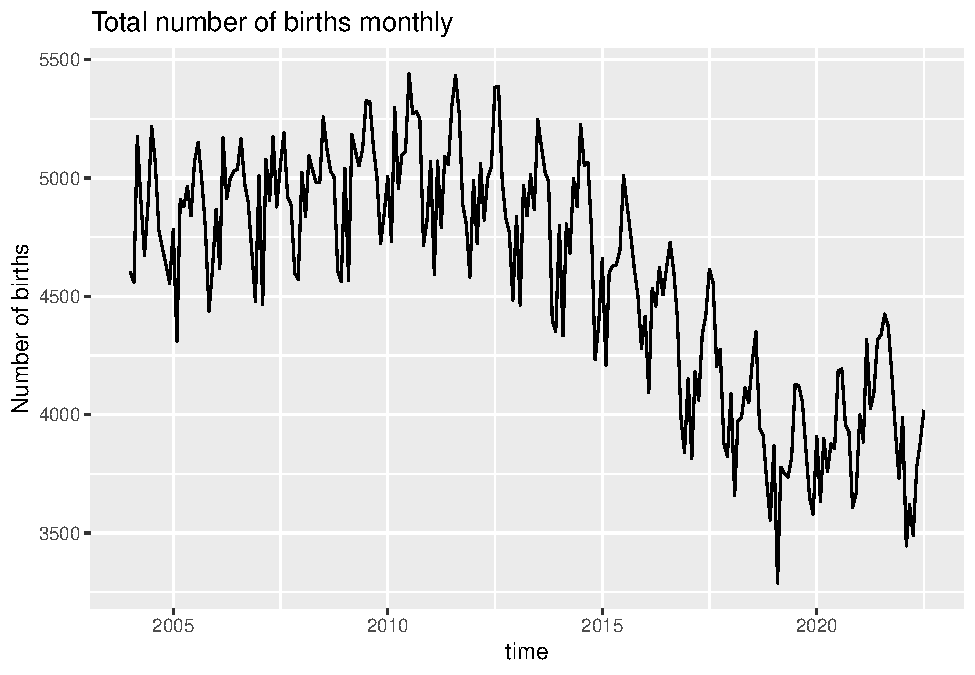
\includegraphics{GoogleTrendsMarkdown_files/figure-latex/unnamed-chunk-2-1.pdf}

\begin{Shaded}
\begin{Highlighting}[]
\FunctionTok{ggplot}\NormalTok{(birthdata, }\FunctionTok{aes}\NormalTok{(}\AttributeTok{x=}\NormalTok{timestamp, }\AttributeTok{y=}\NormalTok{first)) }\SpecialCharTok{+} \FunctionTok{geom\_line}\NormalTok{() }\SpecialCharTok{+} \FunctionTok{labs}\NormalTok{(}\AttributeTok{x=}\StringTok{"time"}\NormalTok{, }\AttributeTok{y=}\StringTok{"Number of births"}\NormalTok{, }\AttributeTok{title=}\StringTok{"Number of firstborns monthly"}\NormalTok{) }
\end{Highlighting}
\end{Shaded}

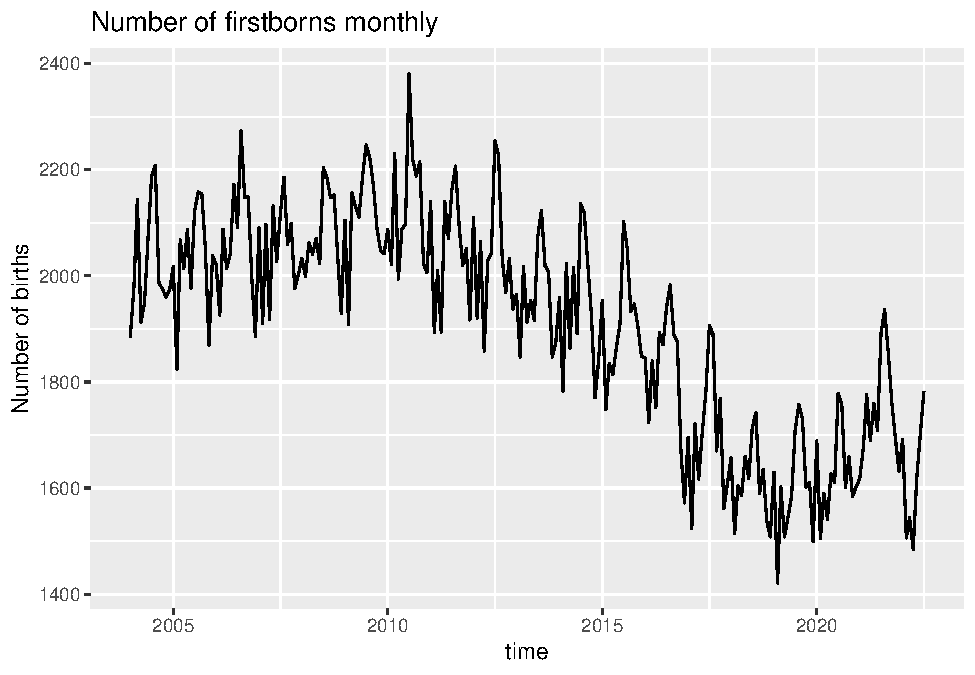
\includegraphics{GoogleTrendsMarkdown_files/figure-latex/unnamed-chunk-2-2.pdf}

\hypertarget{decomposing-total-births-and-firstborns}{%
\subsubsection{Decomposing total births and
firstborns}\label{decomposing-total-births-and-firstborns}}

\begin{Shaded}
\begin{Highlighting}[]
\NormalTok{births\_total}\OtherTok{\textless{}{-}}\NormalTok{birthdata}\SpecialCharTok{$}\NormalTok{total}
\NormalTok{births\_total }\OtherTok{\textless{}{-}} \FunctionTok{ts}\NormalTok{(births\_total,}\AttributeTok{start=}\FunctionTok{c}\NormalTok{(}\DecValTok{2004}\NormalTok{,}\DecValTok{1}\NormalTok{),}\AttributeTok{end=}\FunctionTok{c}\NormalTok{(}\DecValTok{2022}\NormalTok{,}\DecValTok{7}\NormalTok{),}\AttributeTok{frequency=}\DecValTok{12}\NormalTok{)}
\NormalTok{decomp\_births\_total }\OtherTok{\textless{}{-}} \FunctionTok{decompose}\NormalTok{(births\_total)}
\FunctionTok{plot}\NormalTok{(decomp\_births\_total)}
\end{Highlighting}
\end{Shaded}

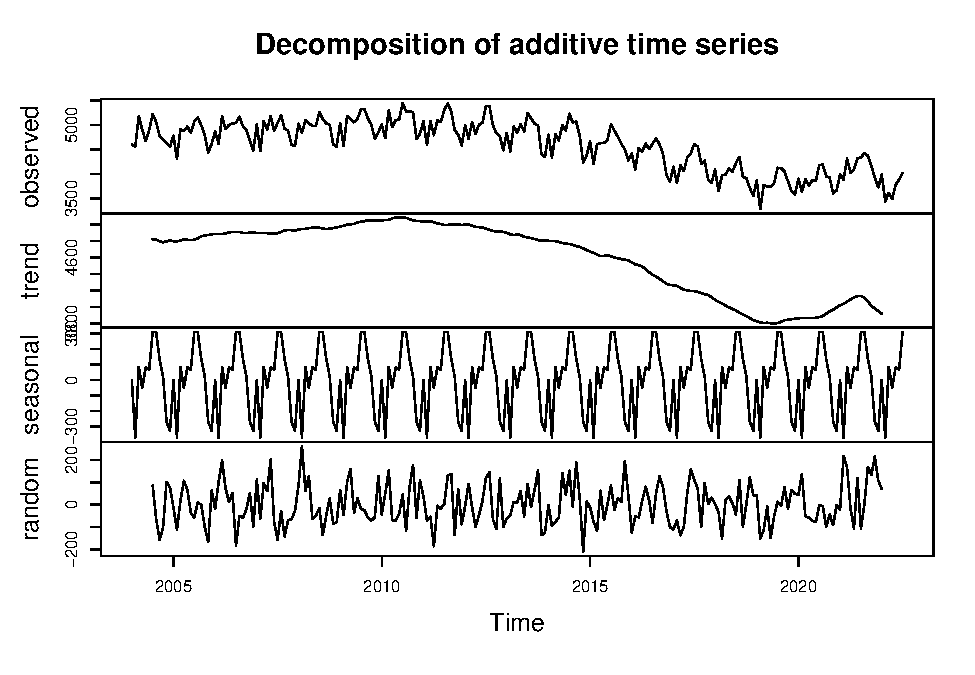
\includegraphics{GoogleTrendsMarkdown_files/figure-latex/unnamed-chunk-3-1.pdf}

\begin{Shaded}
\begin{Highlighting}[]
\NormalTok{births\_firstborn}\OtherTok{\textless{}{-}}\NormalTok{birthdata}\SpecialCharTok{$}\NormalTok{first}
\NormalTok{births\_firstborn }\OtherTok{\textless{}{-}} \FunctionTok{ts}\NormalTok{(births\_firstborn,}\AttributeTok{start=}\FunctionTok{c}\NormalTok{(}\DecValTok{2004}\NormalTok{,}\DecValTok{1}\NormalTok{),}\AttributeTok{end=}\FunctionTok{c}\NormalTok{(}\DecValTok{2022}\NormalTok{,}\DecValTok{7}\NormalTok{),}\AttributeTok{frequency=}\DecValTok{12}\NormalTok{)}
\NormalTok{decomp\_births\_firstborn }\OtherTok{\textless{}{-}} \FunctionTok{decompose}\NormalTok{(births\_firstborn)}
\FunctionTok{plot}\NormalTok{(decomp\_births\_firstborn)}
\end{Highlighting}
\end{Shaded}

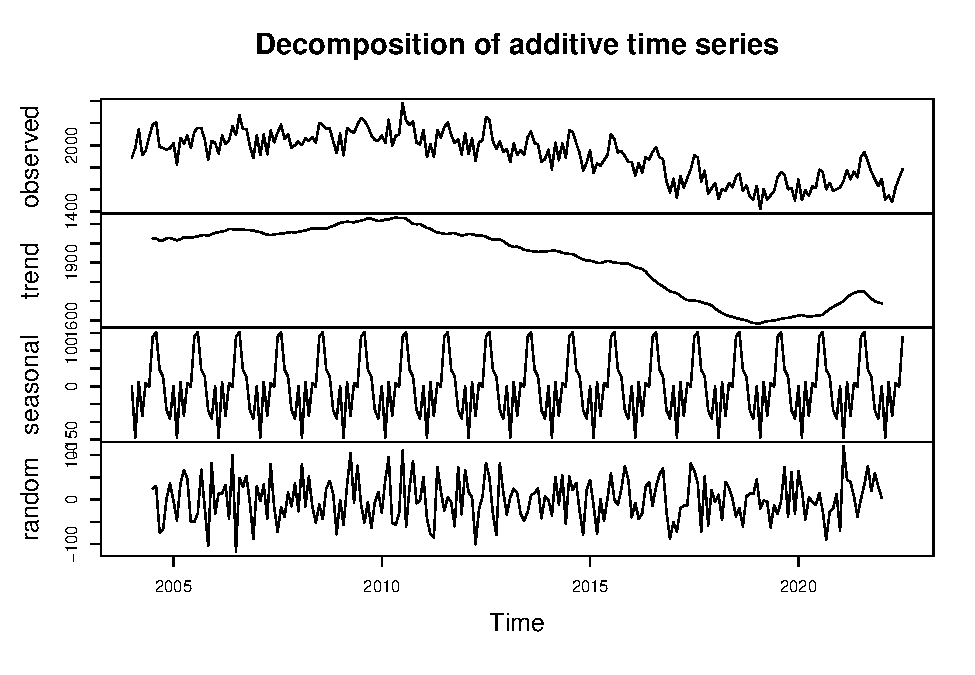
\includegraphics{GoogleTrendsMarkdown_files/figure-latex/unnamed-chunk-3-2.pdf}

\hypertarget{seasonally-adjusting-total-births-and-comparing-it-to-unadjusted-data}{%
\subsubsection{Seasonally adjusting total births and comparing it to
unadjusted
data}\label{seasonally-adjusting-total-births-and-comparing-it-to-unadjusted-data}}

\begin{Shaded}
\begin{Highlighting}[]
\NormalTok{births\_total\_seasonadj }\OtherTok{\textless{}{-}}\NormalTok{ births\_total }\SpecialCharTok{{-}}\NormalTok{ decomp\_births\_total}\SpecialCharTok{$}\NormalTok{seasonal}
\FunctionTok{plot.ts}\NormalTok{(births\_total\_seasonadj)}
\end{Highlighting}
\end{Shaded}

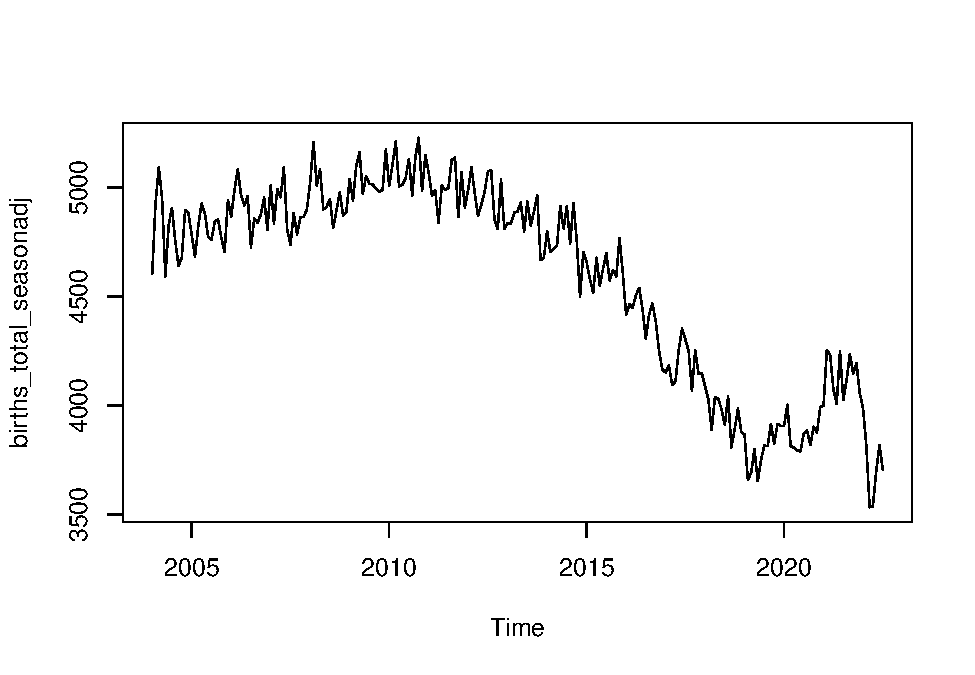
\includegraphics{GoogleTrendsMarkdown_files/figure-latex/unnamed-chunk-4-1.pdf}

\begin{Shaded}
\begin{Highlighting}[]
\FunctionTok{ggplot}\NormalTok{(birthdata, }\FunctionTok{aes}\NormalTok{(}\AttributeTok{x=}\NormalTok{timestamp, }\AttributeTok{y=}\NormalTok{total)) }\SpecialCharTok{+} \FunctionTok{geom\_line}\NormalTok{() }\SpecialCharTok{+} \FunctionTok{labs}\NormalTok{(}\AttributeTok{x=}\StringTok{"time"}\NormalTok{, }\AttributeTok{y=}\StringTok{"Number of births"}\NormalTok{, }\AttributeTok{title=}\StringTok{"Total number of births monthly"}\NormalTok{) }
\end{Highlighting}
\end{Shaded}

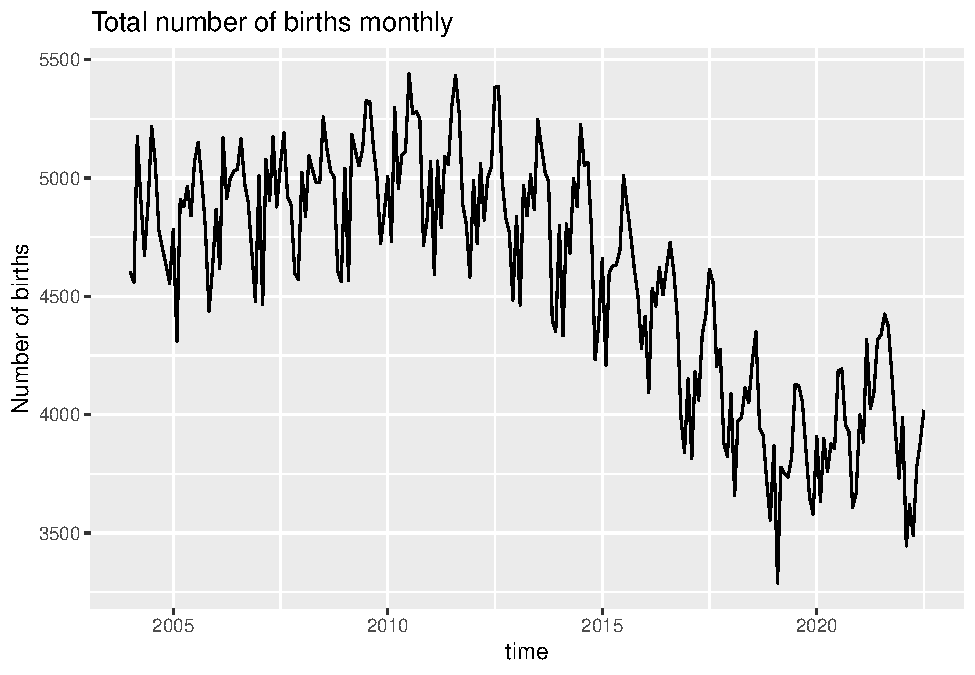
\includegraphics{GoogleTrendsMarkdown_files/figure-latex/unnamed-chunk-4-2.pdf}

\hypertarget{seasonally-adjusting-firstborns-and-comparing-it-to-unadjusted-data}{%
\subsubsection{Seasonally adjusting firstborns and comparing it to
unadjusted
data}\label{seasonally-adjusting-firstborns-and-comparing-it-to-unadjusted-data}}

\begin{Shaded}
\begin{Highlighting}[]
\NormalTok{births\_firstborn\_seasonadj }\OtherTok{\textless{}{-}}\NormalTok{ births\_firstborn }\SpecialCharTok{{-}}\NormalTok{ decomp\_births\_firstborn}\SpecialCharTok{$}\NormalTok{seasonal}
\FunctionTok{plot.ts}\NormalTok{(births\_firstborn\_seasonadj)}
\end{Highlighting}
\end{Shaded}

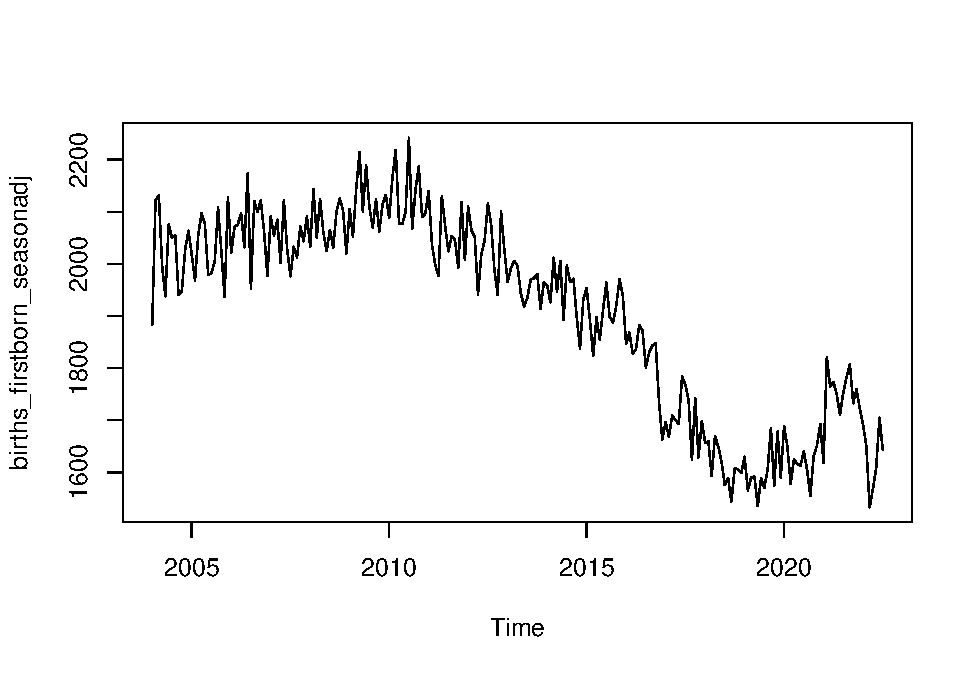
\includegraphics{GoogleTrendsMarkdown_files/figure-latex/unnamed-chunk-5-1.pdf}

\begin{Shaded}
\begin{Highlighting}[]
\FunctionTok{ggplot}\NormalTok{(birthdata, }\FunctionTok{aes}\NormalTok{(}\AttributeTok{x=}\NormalTok{timestamp, }\AttributeTok{y=}\NormalTok{first)) }\SpecialCharTok{+} \FunctionTok{geom\_line}\NormalTok{() }\SpecialCharTok{+} \FunctionTok{labs}\NormalTok{(}\AttributeTok{x=}\StringTok{"time"}\NormalTok{, }\AttributeTok{y=}\StringTok{"Number of births"}\NormalTok{, }\AttributeTok{title=}\StringTok{"Number of firstborns monthly"}\NormalTok{) }
\end{Highlighting}
\end{Shaded}

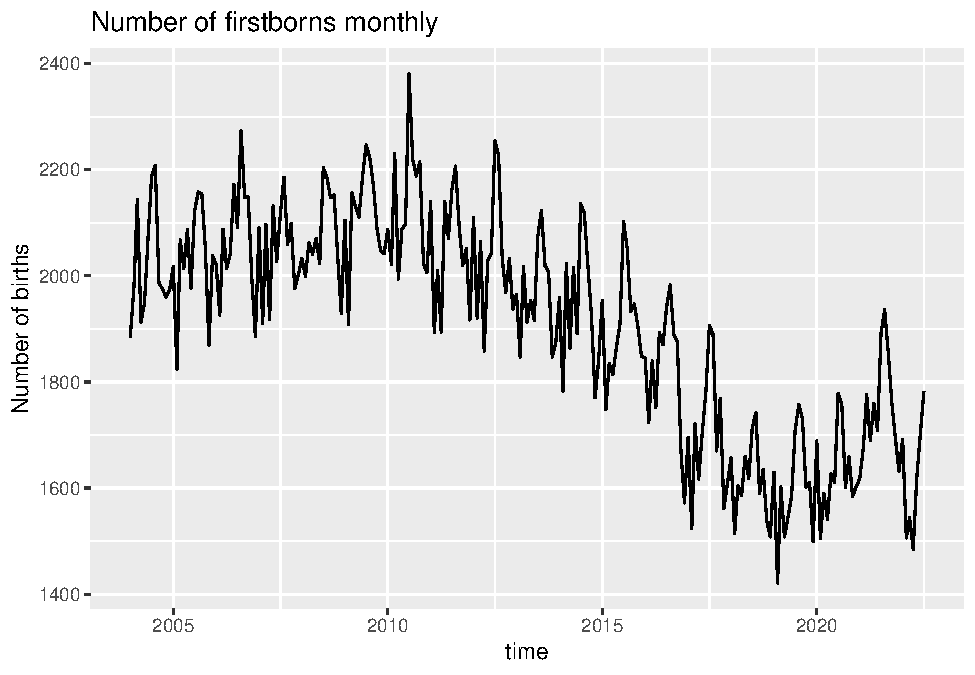
\includegraphics{GoogleTrendsMarkdown_files/figure-latex/unnamed-chunk-5-2.pdf}

\hypertarget{downloading-google-trends-data-for-specified-keywords-and-adjusting-the-seasonality-with-trendecon-package}{%
\subsubsection{Downloading Google trends data for specified keywords and
adjusting the seasonality with TrendEcon
package}\label{downloading-google-trends-data-for-specified-keywords-and-adjusting-the-seasonality-with-trendecon-package}}

\begin{Shaded}
\begin{Highlighting}[]
\DocumentationTok{\#\# Downloading raw data}

\FunctionTok{proc\_keyword\_init}\NormalTok{(}\StringTok{"raskaustesti"}\NormalTok{, }\StringTok{"FI"}\NormalTok{)}
\FunctionTok{proc\_keyword\_init}\NormalTok{(}\StringTok{"clearblue"}\NormalTok{, }\StringTok{"FI"}\NormalTok{)}
\FunctionTok{proc\_keyword\_init}\NormalTok{(}\StringTok{"ovulaatiotesti"}\NormalTok{,}\StringTok{"FI"}\NormalTok{)}
\FunctionTok{proc\_keyword\_init}\NormalTok{(}\StringTok{"raskauspahoinvointi"}\NormalTok{,}\StringTok{"FI"}\NormalTok{)}
\end{Highlighting}
\end{Shaded}

\hypertarget{creating-composite-index-of-the-birth-keywords}{%
\subsubsection{Creating composite index of the birth
keywords}\label{creating-composite-index-of-the-birth-keywords}}

\begin{Shaded}
\begin{Highlighting}[]
\NormalTok{kw\_syntyvyys }\OtherTok{\textless{}{-}} \FunctionTok{c}\NormalTok{(}\StringTok{"raskaustesti"}\NormalTok{,}\StringTok{"clearblue"}\NormalTok{,}\StringTok{"ovulaatiotesti"}\NormalTok{,}\StringTok{"raskauspahoinvointi"}\NormalTok{)}

\CommentTok{\#proc\_index(kw\_syntyvyys,"FI","syntyvyysindex")}
\end{Highlighting}
\end{Shaded}

\hypertarget{importing-seasonally-adjusted-data-of-keywords-and-turning-it-to-monthly-data}{%
\subsubsection{Importing seasonally adjusted data of keywords and
turning it to monthly
data}\label{importing-seasonally-adjusted-data-of-keywords-and-turning-it-to-monthly-data}}

\begin{Shaded}
\begin{Highlighting}[]
\NormalTok{raskaustesti\_sa }\OtherTok{\textless{}{-}} \FunctionTok{read\_csv}\NormalTok{(}\StringTok{"raw/fi/raskaustesti\_sa.csv"}\NormalTok{, }\AttributeTok{col\_types =} \FunctionTok{cols}\NormalTok{(}\AttributeTok{time =} \FunctionTok{col\_date}\NormalTok{(}\AttributeTok{format =} \StringTok{"\%Y{-}\%m{-}\%d"}\NormalTok{)))}
\NormalTok{raskaustesti\_sa}\SpecialCharTok{$}\NormalTok{month }\OtherTok{\textless{}{-}} \FunctionTok{floor\_date}\NormalTok{(raskaustesti\_sa}\SpecialCharTok{$}\NormalTok{time, }\StringTok{"month"}\NormalTok{)}
\NormalTok{raskaustesti\_monthly }\OtherTok{\textless{}{-}}\NormalTok{ (raskaustesti\_sa }\SpecialCharTok{\%\textgreater{}\%} \FunctionTok{group\_by}\NormalTok{(month) }\SpecialCharTok{\%\textgreater{}\%} \FunctionTok{summarize}\NormalTok{(}\AttributeTok{mean =} \FunctionTok{mean}\NormalTok{(value)))}

\NormalTok{clearblue\_sa }\OtherTok{\textless{}{-}} \FunctionTok{read\_csv}\NormalTok{(}\StringTok{"raw/fi/clearblue\_sa.csv"}\NormalTok{, }\AttributeTok{col\_types =} \FunctionTok{cols}\NormalTok{(}\AttributeTok{time=}\FunctionTok{col\_date}\NormalTok{(}\AttributeTok{format =} \StringTok{"\%Y{-}\%m{-}\%d"}\NormalTok{)))}
\NormalTok{clearblue\_sa}\SpecialCharTok{$}\NormalTok{month }\OtherTok{\textless{}{-}} \FunctionTok{floor\_date}\NormalTok{(clearblue\_sa}\SpecialCharTok{$}\NormalTok{time, }\StringTok{"month"}\NormalTok{)}
\NormalTok{clearblue\_monthly }\OtherTok{\textless{}{-}}\NormalTok{ (clearblue\_sa }\SpecialCharTok{\%\textgreater{}\%} \FunctionTok{group\_by}\NormalTok{(month) }\SpecialCharTok{\%\textgreater{}\%} \FunctionTok{summarize}\NormalTok{(}\AttributeTok{mean =} \FunctionTok{mean}\NormalTok{(value)))}

\NormalTok{ovulaatiotesti\_sa }\OtherTok{\textless{}{-}} \FunctionTok{read\_csv}\NormalTok{(}\StringTok{"raw/fi/ovulaatiotesti\_sa.csv"}\NormalTok{, }\AttributeTok{col\_types =} \FunctionTok{cols}\NormalTok{(}\AttributeTok{time=}\FunctionTok{col\_date}\NormalTok{(}\AttributeTok{format =} \StringTok{"\%Y{-}\%m{-}\%d"}\NormalTok{)))}
\NormalTok{ovulaatiotesti\_sa}\SpecialCharTok{$}\NormalTok{month }\OtherTok{\textless{}{-}} \FunctionTok{floor\_date}\NormalTok{(ovulaatiotesti\_sa}\SpecialCharTok{$}\NormalTok{time, }\StringTok{"month"}\NormalTok{)}
\NormalTok{ovulaatiotesti\_monthly }\OtherTok{\textless{}{-}}\NormalTok{ (ovulaatiotesti\_sa }\SpecialCharTok{\%\textgreater{}\%} \FunctionTok{group\_by}\NormalTok{(month) }\SpecialCharTok{\%\textgreater{}\%} \FunctionTok{summarize}\NormalTok{(}\AttributeTok{mean =} \FunctionTok{mean}\NormalTok{(value)))}

\NormalTok{raskauspahoinvointi\_sa }\OtherTok{\textless{}{-}} \FunctionTok{read\_csv}\NormalTok{(}\StringTok{"raw/fi/raskauspahoinvointi\_sa.csv"}\NormalTok{, }\AttributeTok{col\_types =} \FunctionTok{cols}\NormalTok{(}\AttributeTok{time=}\FunctionTok{col\_date}\NormalTok{(}\AttributeTok{format =} \StringTok{"\%Y{-}\%m{-}\%d"}\NormalTok{)))}
\NormalTok{raskauspahoinvointi\_sa}\SpecialCharTok{$}\NormalTok{month }\OtherTok{\textless{}{-}} \FunctionTok{floor\_date}\NormalTok{(raskauspahoinvointi\_sa}\SpecialCharTok{$}\NormalTok{time, }\StringTok{"month"}\NormalTok{)}
\NormalTok{raskauspahoinvointi\_monthly }\OtherTok{\textless{}{-}}\NormalTok{ (raskauspahoinvointi\_sa }\SpecialCharTok{\%\textgreater{}\%} \FunctionTok{group\_by}\NormalTok{(month) }\SpecialCharTok{\%\textgreater{}\%} \FunctionTok{summarize}\NormalTok{(}\AttributeTok{mean =} \FunctionTok{mean}\NormalTok{(value)))}
\end{Highlighting}
\end{Shaded}

\hypertarget{plotting-the-individual-seasonally-adjusted-keywords-on-monthly-level}{%
\subsubsection{Plotting the individual seasonally adjusted keywords on
monthly
level}\label{plotting-the-individual-seasonally-adjusted-keywords-on-monthly-level}}

\begin{Shaded}
\begin{Highlighting}[]
\FunctionTok{ggplot}\NormalTok{(raskaustesti\_monthly, }\FunctionTok{aes}\NormalTok{(}\AttributeTok{x=}\NormalTok{month,}\AttributeTok{y=}\NormalTok{mean)) }\SpecialCharTok{+} \FunctionTok{labs}\NormalTok{(}\AttributeTok{title=}\StringTok{"Seasonally adjusted keyword index for raskaustesti"}\NormalTok{) }\SpecialCharTok{+} \FunctionTok{geom\_line}\NormalTok{()}
\end{Highlighting}
\end{Shaded}

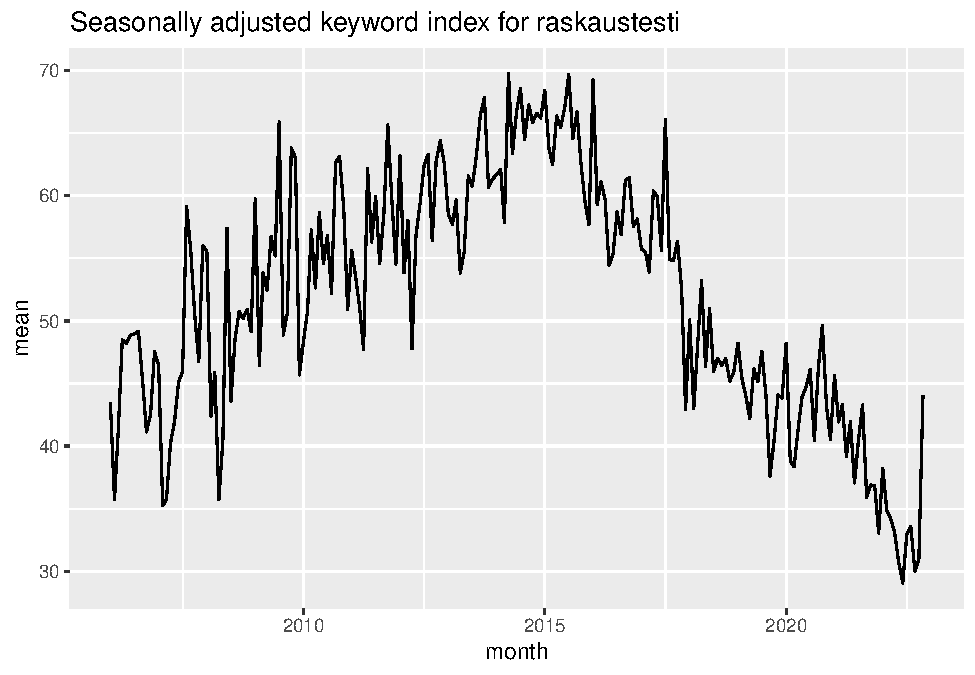
\includegraphics{GoogleTrendsMarkdown_files/figure-latex/unnamed-chunk-9-1.pdf}

\begin{Shaded}
\begin{Highlighting}[]
\FunctionTok{ggplot}\NormalTok{(clearblue\_monthly, }\FunctionTok{aes}\NormalTok{(}\AttributeTok{x=}\NormalTok{month,}\AttributeTok{y=}\NormalTok{mean)) }\SpecialCharTok{+} \FunctionTok{labs}\NormalTok{(}\AttributeTok{title=}\StringTok{"Seasonally adjusted keyword index for clearblue"}\NormalTok{) }\SpecialCharTok{+} \FunctionTok{geom\_line}\NormalTok{()}
\end{Highlighting}
\end{Shaded}

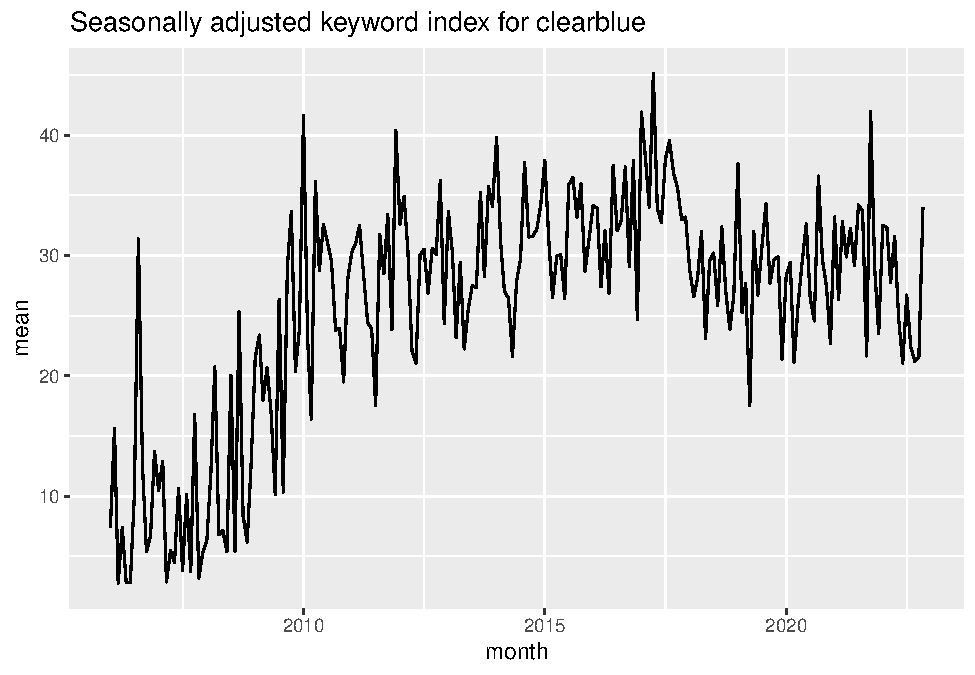
\includegraphics{GoogleTrendsMarkdown_files/figure-latex/unnamed-chunk-9-2.pdf}

\begin{Shaded}
\begin{Highlighting}[]
\FunctionTok{ggplot}\NormalTok{(ovulaatiotesti\_monthly, }\FunctionTok{aes}\NormalTok{(}\AttributeTok{x=}\NormalTok{month,}\AttributeTok{y=}\NormalTok{mean)) }\SpecialCharTok{+} \FunctionTok{labs}\NormalTok{(}\AttributeTok{title=}\StringTok{"Seasonally adjusted keyword index for ovulaatiotesti"}\NormalTok{) }\SpecialCharTok{+} \FunctionTok{geom\_line}\NormalTok{()}
\end{Highlighting}
\end{Shaded}

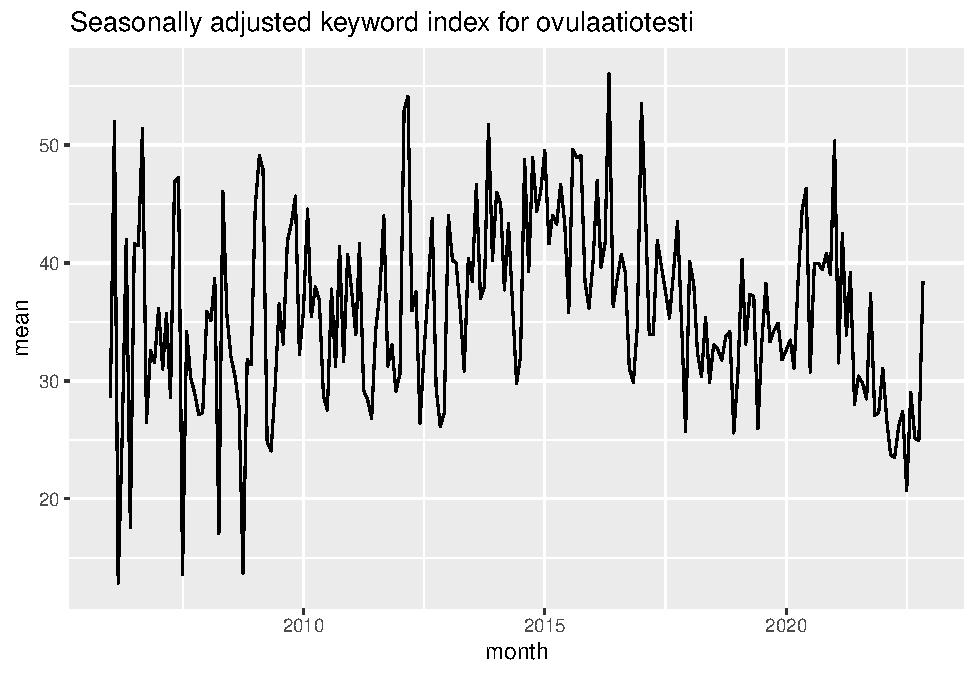
\includegraphics{GoogleTrendsMarkdown_files/figure-latex/unnamed-chunk-9-3.pdf}

\begin{Shaded}
\begin{Highlighting}[]
\FunctionTok{ggplot}\NormalTok{(raskauspahoinvointi\_monthly, }\FunctionTok{aes}\NormalTok{(}\AttributeTok{x=}\NormalTok{month,}\AttributeTok{y=}\NormalTok{mean)) }\SpecialCharTok{+} \FunctionTok{labs}\NormalTok{(}\AttributeTok{title=}\StringTok{"Seasonally adjusted keyword index for raskauspahoinvointi"}\NormalTok{) }\SpecialCharTok{+} \FunctionTok{geom\_line}\NormalTok{()}
\end{Highlighting}
\end{Shaded}

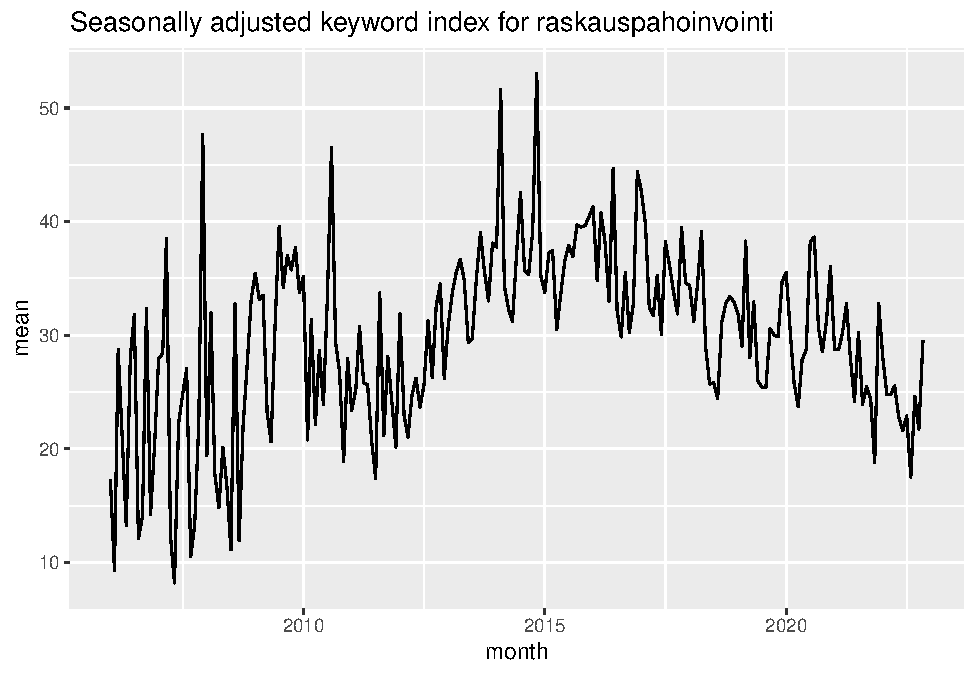
\includegraphics{GoogleTrendsMarkdown_files/figure-latex/unnamed-chunk-9-4.pdf}

\hypertarget{creating-index-for-multiple-keywords-and-plotting-the-index-and-for-comparison-the-total-births-index}{%
\subsubsection{Creating index for multiple keywords and plotting the
index and for comparison the total births
index}\label{creating-index-for-multiple-keywords-and-plotting-the-index-and-for-comparison-the-total-births-index}}

\begin{Shaded}
\begin{Highlighting}[]
\NormalTok{syntyvyysindeksi }\OtherTok{\textless{}{-}} \FunctionTok{read\_csv}\NormalTok{(}\StringTok{"raw/fi/syntyvyysindex\_sa.csv"}\NormalTok{, }\AttributeTok{col\_types =} \FunctionTok{cols}\NormalTok{(}\AttributeTok{time =} \FunctionTok{col\_date}\NormalTok{(}\AttributeTok{format =} \StringTok{"\%Y{-}\%m{-}\%d"}\NormalTok{), }
                                                                              \AttributeTok{value =} \FunctionTok{col\_number}\NormalTok{()))}
\NormalTok{syntyvyysindeksi}\SpecialCharTok{$}\NormalTok{month }\OtherTok{\textless{}{-}} \FunctionTok{floor\_date}\NormalTok{(syntyvyysindeksi}\SpecialCharTok{$}\NormalTok{time, }\StringTok{"month"}\NormalTok{)}
\NormalTok{syntyvyysindeksi }\SpecialCharTok{\%\textgreater{}\%} \FunctionTok{group\_by}\NormalTok{(month) }\SpecialCharTok{\%\textgreater{}\%} \FunctionTok{summarize}\NormalTok{(}\AttributeTok{mean =} \FunctionTok{mean}\NormalTok{(value))}
\end{Highlighting}
\end{Shaded}

\begin{verbatim}
## # A tibble: 203 x 2
##    month         mean
##    <date>       <dbl>
##  1 2006-01-01 -2.10  
##  2 2006-02-01 -1.20  
##  3 2006-03-01 -1.85  
##  4 2006-04-01 -0.976 
##  5 2006-05-01 -1.14  
##  6 2006-06-01 -1.15  
##  7 2006-07-01  0.0155
##  8 2006-08-01 -0.215 
##  9 2006-09-01 -0.685 
## 10 2006-10-01 -1.19  
## # ... with 193 more rows
\end{verbatim}

\begin{Shaded}
\begin{Highlighting}[]
\NormalTok{syntyvyysindeksi\_monthly }\OtherTok{\textless{}{-}}\NormalTok{ (syntyvyysindeksi }\SpecialCharTok{\%\textgreater{}\%} \FunctionTok{group\_by}\NormalTok{(month) }\SpecialCharTok{\%\textgreater{}\%} \FunctionTok{summarize}\NormalTok{(}\AttributeTok{mean =} \FunctionTok{mean}\NormalTok{(value)))}

\FunctionTok{ggplot}\NormalTok{(syntyvyysindeksi\_monthly, }\FunctionTok{aes}\NormalTok{(}\AttributeTok{x=}\NormalTok{month,}\AttributeTok{y=}\NormalTok{mean)) }\SpecialCharTok{+} \FunctionTok{labs}\NormalTok{(}\AttributeTok{title=}\StringTok{"Seasonally adjusted index for birth related keywords"}\NormalTok{) }\SpecialCharTok{+} \FunctionTok{geom\_line}\NormalTok{()}
\end{Highlighting}
\end{Shaded}

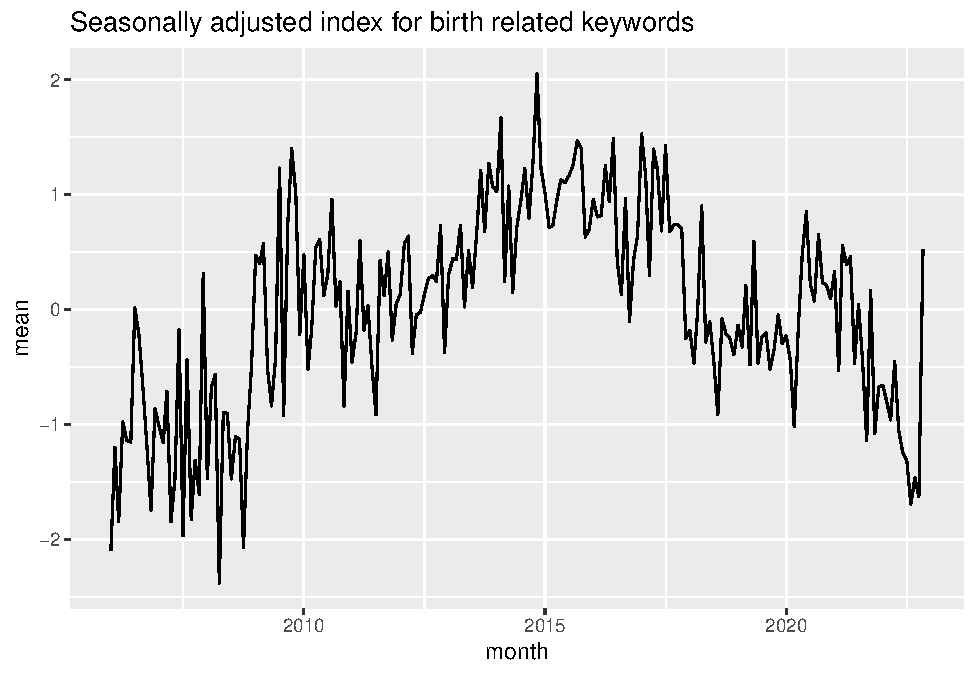
\includegraphics{GoogleTrendsMarkdown_files/figure-latex/unnamed-chunk-10-1.pdf}

\begin{Shaded}
\begin{Highlighting}[]
\FunctionTok{plot.ts}\NormalTok{(births\_total\_seasonadj)}
\end{Highlighting}
\end{Shaded}

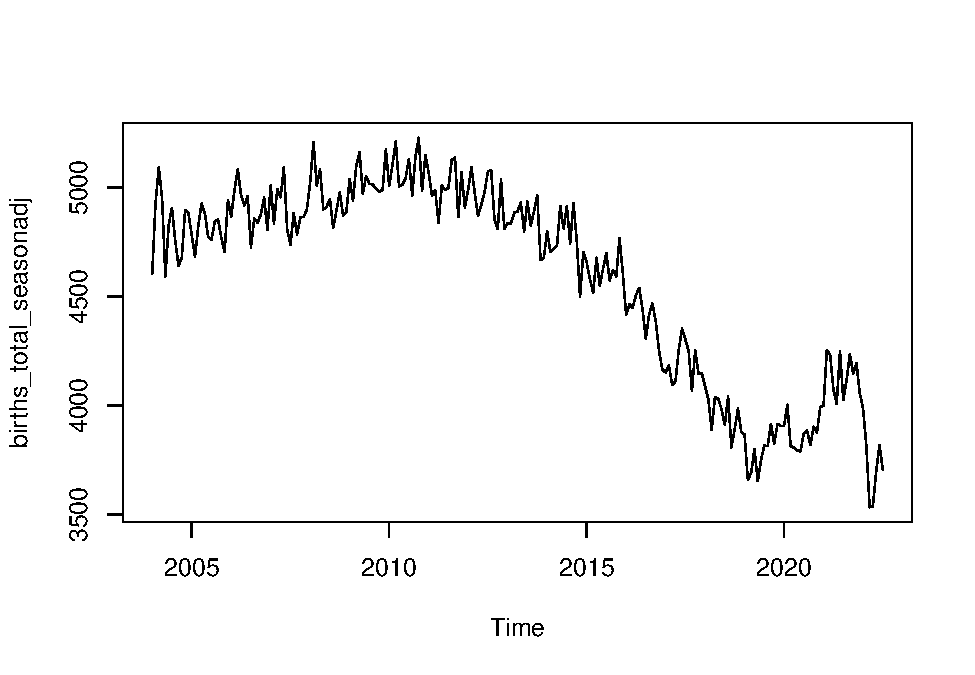
\includegraphics{GoogleTrendsMarkdown_files/figure-latex/unnamed-chunk-10-2.pdf}

\end{document}
